In this section, we explain information about the test problems and corresponding instances in summarized manner. This includes problem type, components (variables and constraints), and instances for each problem.  

\subsection{Type of problems}
Table \ref{table:problems} summarizes the description of each test problem in \siplibtwo. The five of them are adopted from \siplib\ \cite{web:SIPLIB1}. We tried to implement the \siplib\ instances as same as the original references possible. Not all of them, however, are exactly the same due to insufficient information on problem parameters, e.g., random numbers in scenarios. We developed our own way to implement the problems as long as it does not harm the problem's own characteristic. We explain detailed problem-specific information in Section \ref{sec:prob_desc} for those who are interested in.
\begin{table}[H]
	\centering
	\caption{Problems in \texttt{SIPLIB 2.0}}
	\label{table:problems}
	\resizebox{\textwidth}{!}{%
		\begin{tabular}{@{}llll@{}}
			\toprule
			Problem		  		  & Description                                                        & Main reference              \\ \midrule
			\texttt{DCAP}         & Dynamic capacity planning with stochastic demand \ref{DCAP}                   & Ahmed and Garcia \cite{journal:AG2004}                          \\
			\texttt{DCLP}		  &	Data center location problem	\ref{DCLP}								   & Kim et al. \cite{journal:KYZC2017}								\\	
			\texttt{MPTSPs}       & Multi-path traveling salesman problem with stochastic travel costs \ref{MPTSPs}& Tadei et al. \cite{journal:TPP2017}                            \\
			\texttt{SIZES}        & Optimal product substitution with stochastic demand \ref{SIZES}         & Jorjani et al. \cite{journal:JSW1999}          \\
			\texttt{SMKP}		  & Stochastic multiple knapsack problem \ref{SMKP}                              & Angulo et al. \cite{journal:AAD2014}                            \\
			\texttt{SSLP}         & Stochastic server location problem \ref{SSLP}                                & Ntaimo and Sen \cite{journal:NS2005}                           \\
			\texttt{SUCW}         & Wind power stochastic unit commitment	\ref{SUCW}			               & Papavasiliou and Oren \cite{journal:PO2013}                       \\ \bottomrule
		\end{tabular}%
	}
\end{table}

Table \ref{table:naming_rule} shows how we name the instances. The capital Roman letters mean the sets defining the problems and the calligraphic letters mean the scenario sets. For notational convenience, we sometimes skip the cardinality sign $|\cdot|$ for sets, i.e., for any set $S$, $S$ denotes the number of elements $|S|$ in Table \ref{table:naming_rule} and \ref{table:num_components}. Note that not all sets are used to define an instance. The sets that do not appear in the instance name are fixed by some pre-determined value by the original references so we follow them. For example, in \texttt{SMKP} there are 4 sets in total, $I,J,K,\mathcal{S}$, but the numbers of knapsacks $|J|$ and $|K|$ are fixed by 50 and 5.

\begin{table}[H]
	\centering
	\caption{Instance naming rules}
	\label{table:naming_rule}
	\resizebox{\textwidth}{!}{%
		\begin{tabular}{@{}lll@{}}
			\toprule
			Problem & Instance name                 & Remark                                                                    					      \\ \midrule
			\texttt{DCAP}    & \texttt{DCAP\_$R$\_$N$\_$T$\_$\mathcal{S}$}    &   $R$: number of resources, $N$: number of tasks, $T$: number of time periods, $\mathcal{S}$: number of scenarios        \\
			\texttt{DCLP}	 &								&																										\\
			\texttt{MPTSPs}  & \texttt{MPTSPs\_$D$\_$N$\_$\mathcal{S}$} &$D$: node distribution strategy, $N$: number of nodes, $\mathcal{S}$: number of scenarios\\
			\texttt{SIZES}   & \texttt{SIZES\_$\mathcal{S}$}                            & $\mathcal{S}$: number of scenarios   															\\
			\texttt{SMKP}    &   \texttt{SMKP\_$I$\_$\mathcal{S}$}    &   $I$:number of types for item, $\mathcal{S}$: number of scenarios  													 \\
			\texttt{SSLP}    &   \texttt{SSLP\_$I$\_$J$\_$\mathcal{S}$}      &    $I$: number of clients, $J$: number of server locations, $\mathcal{S}$: number of scenarios                 				   \\
			\texttt{SUCW}    & 	\texttt{SUCW\_$D$\_$\mathcal{S}$}    &  $D$: day type, $\mathcal{S}$: number of scenarios                                                 						 \\ \bottomrule
		\end{tabular}%
	}
\end{table}

In \siplibtwo\, we mainly classify each problem by its stage-wise variable types. We consider three types of variable: continuous, binary, and integer. Considering two stages, the possible number of combination is $\left[\sum_{k=1}^3\binom{3}{k}\right]^2=49$ in total. We try to include problems with non-overlapping such combination. Table \ref{table:prob_class} shows the stage-wise components (variable and constraints) of each problem. For the abbreviated notation on the constraints, we refer \texttt{MIPLIB 2010} \cite{MIPLIB}. Although the constraint type is possibly one of the important factors that define the problem characteristic, we decided not to consider it for classification and let this future work since it can cause too much varieties, which we cannot easily capture the insight from the problem type classification. 
\begin{table}[H]
	\centering
	\caption{Components of the problems}
	\label{table:prob_class}
	\begin{threeparttable}
		\begin{tabular}{@{}lllll@{}}
			\toprule
			& \multicolumn{2}{l}{1st stage}                              				  	& \multicolumn{2}{l}{2nd stage}                             			        \\ \midrule
			Problem 	     & Variable                    & Constraint                   	& Variable                    & Constraint                  				    \\ \midrule
			\texttt{DCAP}    & $\mathbb{C}$, $\mathbb{B}$  & \texttt{VBB}                	& $\mathbb{B}$                & \texttt{PAR}, \texttt{M01} 			    		\\
			\texttt{DCLP}	 &							   &								& 			 	  &													\\				
			\texttt{MPTSPs}  & $\mathbb{C}$, $\mathbb{B}$  & \texttt{PAR}, \texttt{GEN}		& $\mathbb{B}$                & \texttt{GEN}               						\\
			\texttt{SIZES}   & $\mathbb{I}$ 			   & \texttt{VBD}, \texttt{GEN} 	& $\mathbb{B}$, $\mathbb{I}$  & \texttt{IKN}             						\\
			\texttt{SMKP}    & $\mathbb{B}$                & \texttt{KNA}                	& $\mathbb{B}$                & \texttt{KNA}              						\\
			\texttt{SSLP}    & $\mathbb{B}$                & \texttt{IVK}, \texttt{GEN} 	& $\mathbb{C}$, $\mathbb{B}$  & \texttt{GEN}             						\\
			\texttt{SUCW}    & $\mathbb{C}$, $\mathbb{B}$                 &                              	& $\mathbb{C}$, $\mathbb{B}$  &                             					\\ \bottomrule
		\end{tabular}
		
		\begin{tablenotes}
			\small
			\item $\mathbb{C}$: continuous, $\mathbb{B}$: binary, $\mathbb{I}$: integer
		\end{tablenotes}
	\end{threeparttable}
\end{table}

Table 

%\begin{table}[H]
%	\centering
%	\caption{Constraint type legend \cite{MIPLIB}}
%	\label{table:constraint_type}
%	\begin{tabular}{@{}lll@{}}
%		\toprule
%		Type           & Description        & Constraint form                                                                                           \\ \midrule
%		\texttt{AGG} & Aggregation        & $a_i x_i+a_k x_k=b,\ x_i , x_k$ int. or cont., $a_i , a_k , b \in \mathbb{R}$                  \\
%		\texttt{VBD} & Variable bound     & $x_i \le a_k x_k + b$ or $x_i\ge a_k x_k + b$, $x_i, x_k$ int. or cont., $a_k, b\in\mathbb{R}$ \\
%		\texttt{PAR} & Set partition      & $\sum x_i = 1,$ $x_i$ binary                                                                   \\
%		\texttt{PAC} & Set packing        & $\sum x_i \le 1,$ $x_i$ binary                                                                 \\
%		\texttt{COV} & Set cover          & $\sum x_i \ge 1,$ $x_i$ binary                                                                 \\
%		\texttt{CAR} & Cardinality        & $\sum x_i = b,$ $x_i$ binary, $b\in\mathbb{N}$                                                 \\
%		\texttt{EQK} & Equality knapsack  & $\sum a_i x_i = b,$ $x_i$ binary, $a_i , b\in\mathbb{N}$                                       \\
%		\texttt{BIN} & Bin packing        & $\sum a_i x_i  + a_k x_k \le a_k,$ $x_i$ binary, $a_i , a_k\in\mathbb{N}$                      \\
%		\texttt{IVK} & Invariant knapsack & $\sum x_i \le b,$ $x_i$ binary, $b\in\mathbb{N}$                                               \\
%		\texttt{KNA} & Knapsack           & $a_i x_i \le b$, $x_i$ binary, $a_i,b\in\mathbb{N}$                                            \\
%		\texttt{IKN} & Integer knapsack   & $a_i x_i \le b$, $x_i\ge 0$ integer, $a_i,b\in\mathbb{N}$                                      \\
%		\texttt{M01} & Mixed binary       & $\sum a_i x_i + \sum p_j s_j \le$ or $=b$, $x_i$ binary, $s_j$ cont., $a_i, p_j\in\mathbb{R}$  \\
%		\texttt{GEN} & General            & All other constraint types                                                                     \\ \bottomrule
%	\end{tabular}
%\end{table}



\begin{table}[H]
	\centering
	\resizebox{\textwidth}{!}{%
		\begin{threeparttable}
			\caption{Number of the components in each problem}
			\label{table:num_components}
			\begin{tabular}{@{}cccccc@{}}
				\toprule
				&               & \multicolumn{4}{c}{Components}                                                                         \\ \cmidrule(l){3-6} 
				&                & \#Continuous   & \#Binary                           & \#Integer            & \#Constraint              \\ \midrule
				\multirow{3}{*}{\texttt{DCAP}}   & 1st stage & $RT$           & $RT$                               & -                    & $RT$                      \\
				& 2nd stage & -              & $\left(1+R\right)NT$               & -                    & $(R+N)T$                  \\ \cmidrule(l){2-6} 
				& Total          & $RT$           & $RT+\left(1+R\right)NT\mathcal{S}$ & -                    & $RT+(R+N)T\mathcal{S}$    \\ \midrule
				\multirow{3}{*}{\texttt{DCLP}}   & 1st stage &                &                                    &                      &                           \\
				& 2nd stage &                &                                    &                      &                           \\ \cmidrule(l){2-6} 
				& Total          &                &                                    &                      &                           \\ \midrule
				\multirow{3}{*}{\texttt{MPTSPs}} & 1st stage & $(N-1)N$          & $(N-1)N$                              & -                    & $N^2+2N-1$                \\
				& 2nd stage & -              & $(N-1)NK$                            & -                    & $(N-1)N$                     \\ \cmidrule(l){2-6} 
				& Total          & $(N-1)N$          & $(N-1)(1+K\mathcal{S})N$              & -                    & $(1+\mathcal{S})N^2+(2-\mathcal{S})N-1$ \\ \midrule
				\multirow{3}{*}{\texttt{SIZES}}  & 1st stage & -              & $NT$                               & $NT$                 & $(1+N)T$                  \\
				& 2nd stage & -              & -                                  & $N^2 T$              & $2NT$                     \\ \cmidrule(l){2-6} 
				& Total          & -              & $NT$                               & $(1+N\mathcal{S})NT$ & $(1+N+2N\mathcal{S})T$    \\ \midrule
				\multirow{3}{*}{\texttt{SMKP}}   & 1st stage & -              & $2I$                               & -                    & $J$                       \\
				& 2nd stage & -              & $I$                                & -                    & $K$                       \\ \cmidrule(l){2-6} 
				& Total          & -              & $(2+\mathcal{S})I$                 & -                    & $J+K\mathcal{S}$          \\ \midrule
				\multirow{3}{*}{\texttt{SSLP}}   & 1st stage & -              & $J$                                & -                    & $1$                       \\
				& 2nd stage & $J$            & $IJ$                               & -                    & $I+J$                     \\ \cmidrule(l){2-6} 
				& Total          & $J\mathcal{S}$ & $(1+I\mathcal{S})J$                & -                    & $1+(I+J)\mathcal{S}$      \\ \midrule
				\multirow{3}{*}{\texttt{SUCW}}   & 1st stage &                &                                    &                      &                           \\
				& 2nd stage &                &                                    &                      &                           \\ \cmidrule(l){2-6} 
				& Total          &                &                                    &                      &                           \\ \bottomrule
			\end{tabular}
	
			\begin{tablenotes}
				\small
				\item For convenience, we skip the cardinality sign $|\cdot|$ for sets, i.e., for any set $S$, $S$ denotes the number of elements $|S|$ in this table.
			\end{tablenotes}
		\end{threeparttable}
	}
\end{table}


\begin{figure}[H]
	\centering
	\subfloat[][\texttt{DCAP\_3\_3\_3\_3}]
	{
		\centering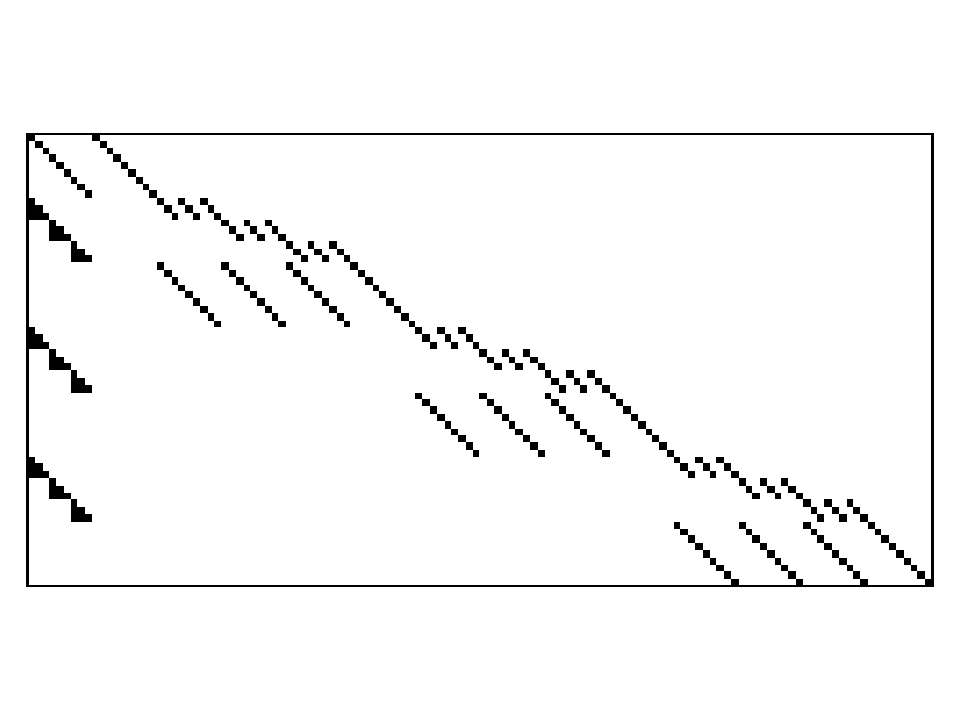
\includegraphics[width=0.45\linewidth]{DCAP_3_3_3_3}
		\label{fig:sparsity_dcap}
	}
	~
	\subfloat[][\texttt{MPTSPs\_D0\_3\_3}]
	{
		\centering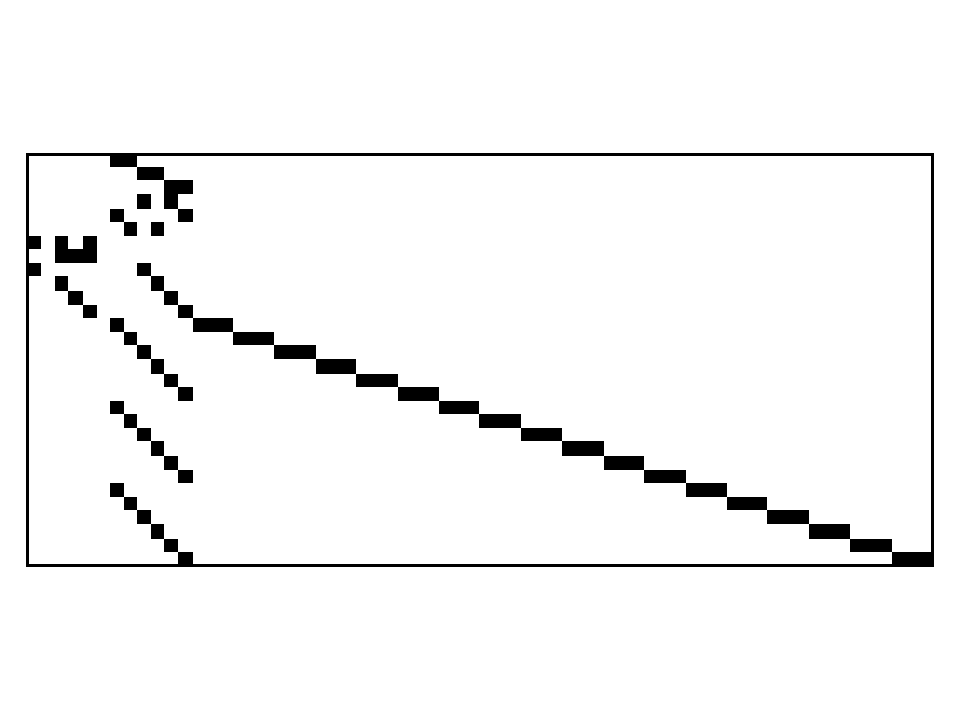
\includegraphics[width=0.45\linewidth]{MPTSPs_D0_3_3}
		\label{fig:sparsity_mptsps}
	}
	
	\subfloat[][\texttt{SIZES\_3}]
	{
		\centering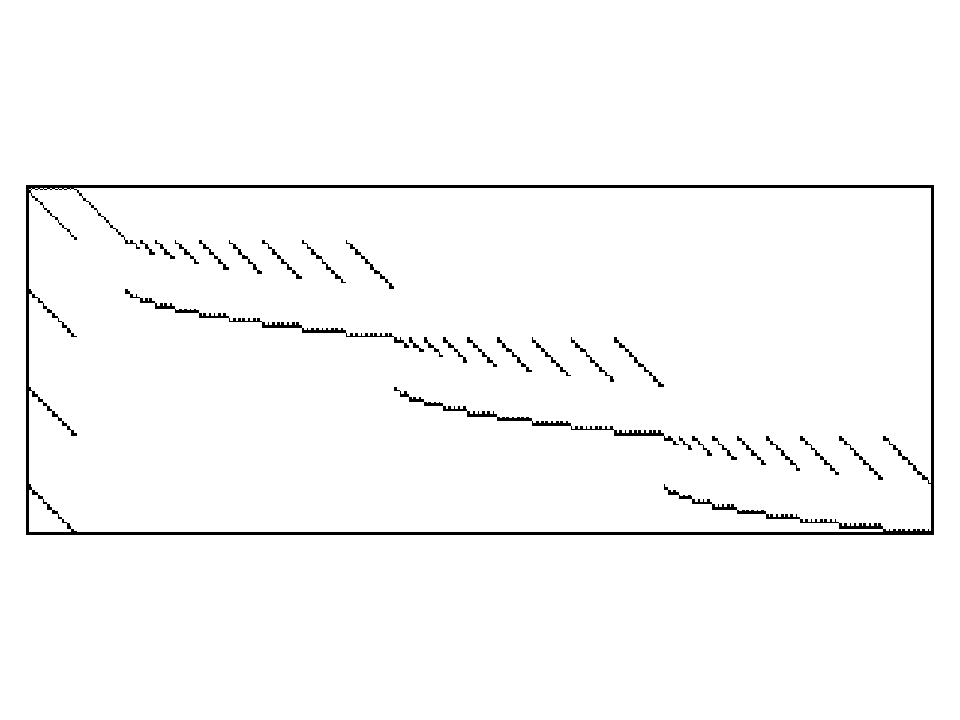
\includegraphics[width=0.45\linewidth]{SIZES_3}
		\label{fig:sparsity_sizes}
	}
	~
	\subfloat[][\texttt{SMKP\_120\_3}]
	{
		\centering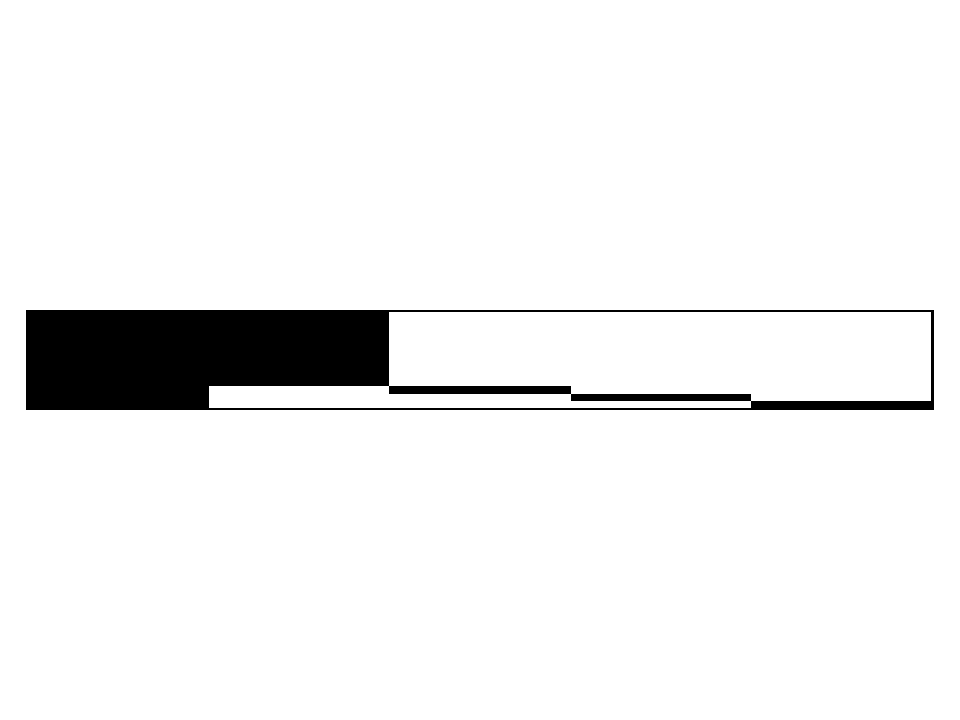
\includegraphics[width=0.45\linewidth]{SMKP_120_3}
		\label{fig:sparsity_smkp}
	}
	
	\subfloat[][\texttt{SSLP\_5\_10\_3}]
	{
		\centering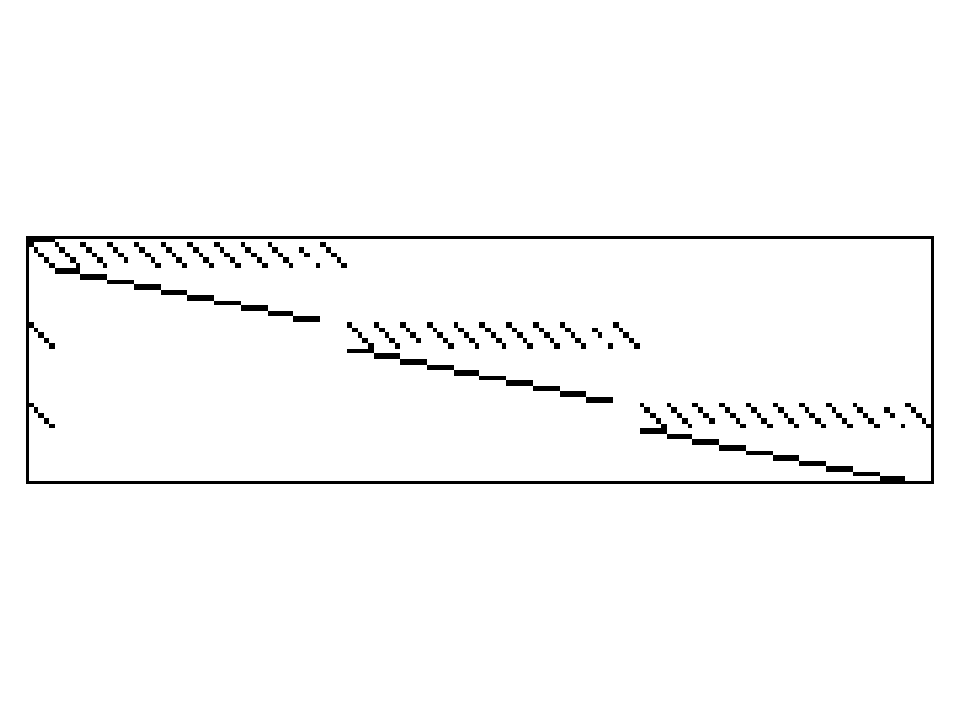
\includegraphics[width=0.45\linewidth]{SSLP_5_10_3}
		\label{fig:sparsity_sslp}
	}
	~
	\subfloat[][\texttt{SUCW\_FallWD\_1}]
	{
		\centering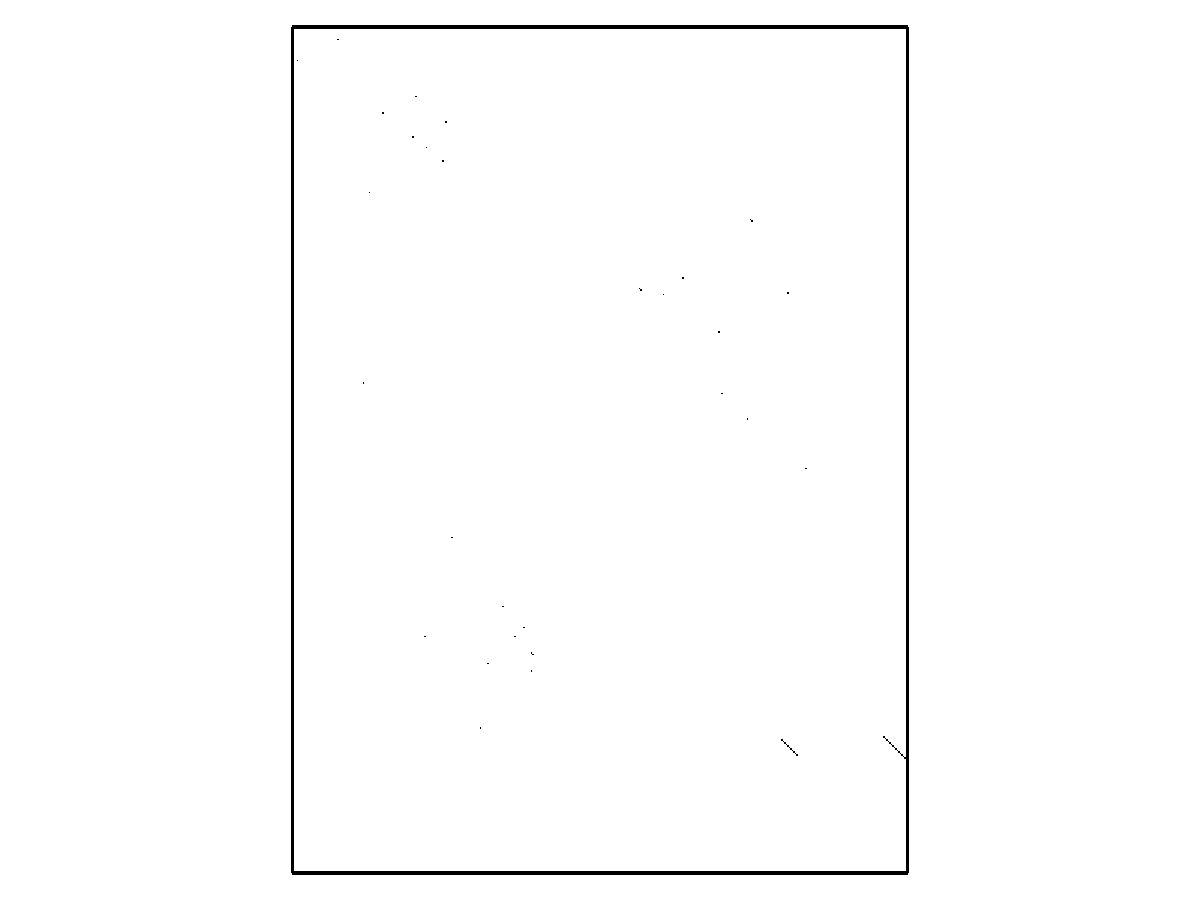
\includegraphics[width=0.45\linewidth]{SUCW_FallWD_1}
		\label{fig:sparsity_sucw}
	}

	\caption{Sparsity pattern for each problem}
	\begin{minipage}
		{0.65\textwidth}{\footnotesize (\texttt{SUCW} instance is too huge and extremely sparse to plot more than 1 scenario)}
	\end{minipage}
	\label{fig:sparsity}
\end{figure}


\subsection{Instance catalog}
% Please add the following required packages to your document preamble:
% \usepackage{multirow}
% \usepackage{graphicx}
%\begin{table}[H]
%	\centering
%	\caption{Size report on the instances}
%	\label{table:instance_size_info}
%%	\resizebox{\textwidth}{!}{%
%		\Rotatebox{90}{%
%		\begin{tabular}{llrrrrrrrrrrrrrlll}
%			\hline
%			&                              & \multicolumn{3}{c}{1st stage variables} & \multicolumn{3}{c}{2nd stage variables} & \multicolumn{7}{c}{Total}                                                 & \multicolumn{3}{c}{File size}                                                  \\ \hline
%			\multicolumn{1}{c}{Problem} & \multicolumn{1}{c}{Instance} & \#cont1      & \#bin1      & \#int1     & \#cont2      & \#bin2      & \#int2     & \#cont  & \#bin    & \#int  & \#rows  & \#cols   & \#nonzeros & \%density & \multicolumn{1}{c}{.cor} & \multicolumn{1}{c}{.tim} & \multicolumn{1}{c}{.sto} \\ \hline
%			\multirow{16}{*}{DCAP}      & DCAP\_2\_3\_3\_500           & 6            & 6           & 0          & 9            & 18          & 0          & 4506    & 9006     & 0      & 7506    & 13512    & 28512      & 0.0281    &                          &                          &                          \\
%			& DCAP\_2\_3\_3\_1000          & 6            & 6           & 0          & 9            & 18          & 0          & 9006    & 18006    & 0      & 15006   & 27012    & 57012      & 0.0141    &                          &                          &                          \\
%			& DCAP\_2\_3\_3\_5000          & 6            & 6           & 0          & 9            & 18          & 0          & 45006   & 90006    & 0      & 75006   & 135012   & 285012     & 0.0028    &                          &                          &                          \\
%			& DCAP\_2\_3\_3\_10000         & 6            & 6           & 0          & 9            & 18          & 0          & 90006   & 180006   & 0      & 150006  & 270012   & 570012     & 0.0014    &                          &                          &                          \\
%			& DCAP\_2\_4\_3\_500           & 6            & 6           & 0          & 12           & 24          & 0          & 6006    & 12006    & 0      & 9006    & 18012    & 36012      & 0.0222    &                          &                          &                          \\
%			& DCAP\_2\_4\_3\_1000          & 6            & 6           & 0          & 12           & 24          & 0          & 12006   & 24006    & 0      & 18006   & 36012    & 72012      & 0.0111    &                          &                          &                          \\
%			& DCAP\_2\_4\_3\_5000          & 6            & 6           & 0          & 12           & 24          & 0          & 60006   & 120006   & 0      & 90006   & 180012   & 360012     & 0.0022    &                          &                          &                          \\
%			& DCAP\_2\_4\_3\_10000         & 6            & 6           & 0          & 12           & 24          & 0          & 120006  & 240006   & 0      & 180006  & 360012   & 720012     & 0.0011    &                          &                          &                          \\
%			& DCAP\_3\_3\_2\_500           & 6            & 6           & 0          & 6            & 18          & 0          & 3006    & 9006     & 0      & 6006    & 12012    & 25512      & 0.0354    &                          &                          &                          \\
%			& DCAP\_3\_3\_2\_1000          & 6            & 6           & 0          & 6            & 18          & 0          & 6006    & 18006    & 0      & 12006   & 24012    & 51012      & 0.0177    &                          &                          &                          \\
%			& DCAP\_3\_3\_2\_5000          & 6            & 6           & 0          & 6            & 18          & 0          & 30006   & 90006    & 0      & 60006   & 120012   & 255012     & 0.0035    &                          &                          &                          \\
%			& DCAP\_3\_3\_2\_10000         & 6            & 6           & 0          & 6            & 18          & 0          & 60006   & 180006   & 0      & 120006  & 240012   & 510012     & 0.0018    &                          &                          &                          \\
%			& DCAP\_3\_4\_2\_500           & 6            & 6           & 0          & 8            & 24          & 0          & 4006    & 12006    & 0      & 7006    & 16012    & 32512      & 0.0290    &                          &                          &                          \\
%			& DCAP\_3\_4\_2\_1000          & 6            & 6           & 0          & 8            & 24          & 0          & 8006    & 24006    & 0      & 14006   & 32012    & 65012      & 0.0145    &                          &                          &                          \\
%			& DCAP\_3\_4\_2\_5000          & 6            & 6           & 0          & 8            & 24          & 0          & 40006   & 120006   & 0      & 70006   & 160012   & 325012     & 0.0029    &                          &                          &                          \\
%			& DCAP\_3\_4\_2\_10000         & 6            & 6           & 0          & 8            & 24          & 0          & 80006   & 240006   & 0      & 140006  & 320012   & 650012     & 0.0015    &                          &                          &                          \\ \hline
%		\end{tabular}%
%%		}
%	}
%\end{table}

% Please add the following required packages to your document preamble:
% \usepackage{multirow}
% \usepackage{graphicx}
\begin{table}[H]
	\centering
	\caption{Size and sparsity report}
	\label{table:instance_size_info}
	%\resizebox{\textwidth}{!}{%
	\Rotatebox{90}{%
		\begin{tabular}{|c|l|lll|lll|lllll|llll|lll|}
			\hline
			\multicolumn{1}{|l|}{} &                               & \multicolumn{3}{c|}{1st stage variables}                                      & \multicolumn{3}{c|}{2nd stage variables (1 scenario)}                         & \multicolumn{5}{c|}{Total size}                                                                                                     & \multicolumn{4}{c|}{Sparsity}                                                                                           & \multicolumn{3}{c|}{File size}                                                  \\ \cline{3-20} 
			Problem                & \multicolumn{1}{c|}{Instance} & \multicolumn{1}{c}{cont} & \multicolumn{1}{c}{bin} & \multicolumn{1}{c|}{int} & \multicolumn{1}{c}{cont} & \multicolumn{1}{c}{bin} & \multicolumn{1}{c|}{int} & \multicolumn{1}{c}{cont} & \multicolumn{1}{c}{bin} & \multicolumn{1}{c}{int} & \multicolumn{1}{c}{rows} & \multicolumn{1}{c|}{cols} & \multicolumn{1}{c}{block A} & \multicolumn{1}{c}{block T} & \multicolumn{1}{c}{block W} & \multicolumn{1}{c|}{In total} & \multicolumn{1}{c}{.cor} & \multicolumn{1}{c}{.tim} & \multicolumn{1}{c|}{.sto} \\ \hline
			\multirow{16}{*}{DCAP} & DCAP\_2\_3\_3\_200            &                          &                         &                          &                          &                         &                          &                          &                         &                         &                          &                           &                             &                             &                             &                               &                          &                          &                           \\
			& DCAP\_2\_3\_3\_300            &                          &                         &                          &                          &                         &                          &                          &                         &                         &                          &                           &                             &                             &                             &                               &                          &                          &                           \\
			& DCAP\_2\_3\_3\_500            &                          &                         &                          &                          &                         &                          &                          &                         &                         &                          &                           &                             &                             &                             &                               &                          &                          &                           \\
			& DCAP\_2\_3\_3\_10000          &                          &                         &                          &                          &                         &                          &                          &                         &                         &                          &                           &                             &                             &                             &                               &                          &                          &                           \\
			& DCAP\_2\_4\_3\_200            &                          &                         &                          &                          &                         &                          &                          &                         &                         &                          &                           &                             &                             &                             &                               &                          &                          &                           \\
			& DCAP\_2\_4\_3\_300            &                          &                         &                          &                          &                         &                          &                          &                         &                         &                          &                           &                             &                             &                             &                               &                          &                          &                           \\
			& DCAP\_2\_4\_3\_500            &                          &                         &                          &                          &                         &                          &                          &                         &                         &                          &                           &                             &                             &                             &                               &                          &                          &                           \\
			& DCAP\_2\_4\_3\_10000          &                          &                         &                          &                          &                         &                          &                          &                         &                         &                          &                           &                             &                             &                             &                               &                          &                          &                           \\
			& DCAP\_3\_3\_2\_200            &                          &                         &                          &                          &                         &                          &                          &                         &                         &                          &                           &                             &                             &                             &                               &                          &                          &                           \\
			& DCAP\_3\_3\_2\_300            &                          &                         &                          &                          &                         &                          &                          &                         &                         &                          &                           &                             &                             &                             &                               &                          &                          &                           \\
			& DCAP\_3\_3\_2\_500            &                          &                         &                          &                          &                         &                          &                          &                         &                         &                          &                           &                             &                             &                             &                               &                          &                          &                           \\
			& DCAP\_3\_3\_2\_10000          &                          &                         &                          &                          &                         &                          &                          &                         &                         &                          &                           &                             &                             &                             &                               &                          &                          &                           \\
			& DCAP\_3\_4\_2\_200            &                          &                         &                          &                          &                         &                          &                          &                         &                         &                          &                           &                             &                             &                             &                               &                          &                          &                           \\
			& DCAP\_3\_4\_2\_300            &                          &                         &                          &                          &                         &                          &                          &                         &                         &                          &                           &                             &                             &                             &                               &                          &                          &                           \\
			& DCAP\_3\_4\_2\_500            &                          &                         &                          &                          &                         &                          &                          &                         &                         &                          &                           &                             &                             &                             &                               &                          &                          &                           \\
			& DCAP\_3\_4\_2\_10000          &                          &                         &                          &                          &                         &                          &                          &                         &                         &                          &                           &                             &                             &                             &                               &                          &                          &                           \\ \hline
		\end{tabular}%
	}
\end{table}



